\documentclass[11pt]{article}
\usepackage{datetime}
\usepackage[T1]{fontenc}
\usepackage{pgfplots}
\usepackage {tikz}
\usetikzlibrary {positioning}
\usepackage{graphicx}


%Gummi|065|=)
\title{\textbf{Lab 4 in C++ OOP}}
\author{Hergeir Winther Lognberg \\
Hewi1600}
\date{}
\usepackage{graphicx}
\begin{document}

\maketitle

\section{Preamble}

The Lab contains folders, each containing an header and corresponding cpp file. The names of the folders correspond to the classes they contain. I'm very sorry for not keeping the main clean, but simply haven't gotten the time.

\subsection{Compilation}
For compiling i use g++ and created a makefile to make the compiling process easier. Just run \emph{"make"} within the lab directory compile.

\section{The Software}
I've tried to keep redundancy away from my code. Each class is only written once and reused in this lab.

Also I have tried to use reference and \emph{const} everywhere it made sense to do so. 

I've tried to use what i've learned so far in an efficient way. I've used an enum called \emph{Algorithm} to keep track of sorting algorithms. Also I've used a struct to bind data together (averageSortingTime,arrayElements and algorithm). Also I created my own Array class from scratch before I read the assignment thoroughly. It dynamically increases and decreases array by deleting and reallocating. I don't have any comment regarding the sorting functions as they where not my creation. I chose to put all timers inside the sorting functions themselves to get rid of function calling-time. 

Would love any feedback on good code practice.

\subsection{Results}
In I've made graphs for all sorting algorithms and included the theoretical graph for each of them. All in all I see that theory is indeed very close to reality i my case. The only algorithms to visibly deviate from theory are BubbleSort and QuickSort (the two extremes). BubbleSort seemed to have some overhead unaccounted for, while quickSort was quicker than theory would allow.
\subsubsection{BubbleSort}	
\begin{center}
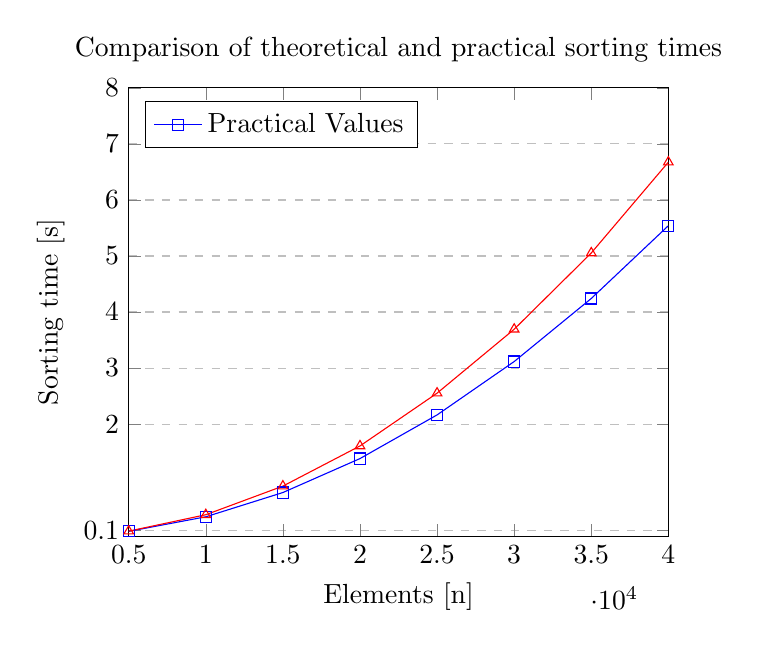
\begin{tikzpicture}
\begin{axis}[
    title={Comparison of theoretical and practical sorting times},
    xlabel={Elements [n]},
    ylabel={Sorting time [s]},
    xmin=5000, xmax=40000,
    ymin=0, ymax=8,
    xtick={0,5000,10000,15000,20000,25000,30000,35000,40000},
    ytick={0.1,2,3,4,5,6,7,8},
    legend pos=north west,
    ymajorgrids=true,
    yminorgrids=true,
    grid style=dashed,
]

\addplot[
    color=blue,
    mark=square,
    ]
    coordinates {
	(5000,0.0865643)(10000,0.3462572)(15000,0.7790786999999999)(20000,1.3850288)(25000,2.1641075)(30000,3.1163147999999996)(35000,4.2416507)(40000,5.5401152)
    };
    \legend{Practical Values}

\addplot[
    color=red,
    mark=triangle,
    ]
    coordinates {
    (5000,0.0901697)(10000,0.383169)(15000,0.893777)(20000,1.6102)(25000,2.55236)(30000,3.6926)(35000,5.05379)(40000,6.67451)
    
    };
  
\end{axis}
\end{tikzpicture}
\end{center}

\subsubsection{SelectionSort}
\begin{center}
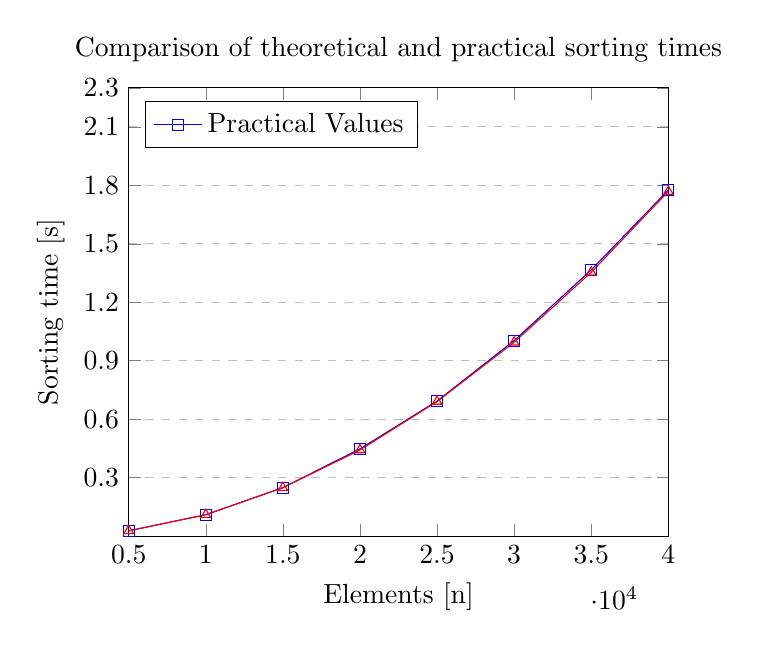
\begin{tikzpicture}
\begin{axis}[
    title={Comparison of theoretical and practical sorting times},
    xlabel={Elements [n]},
    ylabel={Sorting time [s]},
    xmin=5000, xmax=40000,
    ymin=0, ymax=2.3,
    xtick={0,5000,10000,15000,20000,25000,30000,35000,40000},
    ytick={0.3,0.6,0.9,1.2,1.5,1.8,2.1,2.3},
    legend pos=north west,
    ymajorgrids=true,
    yminorgrids=true,
    grid style=dashed,
]

\addplot[
    color=blue,
    mark=square,
    ]
    coordinates {
    (5000,0.0276349)(10000,0.110022)(15000,0.249208)(20000,0.447917)(25000,0.693262)(30000,1.00344)(35000,1.36625)(40000,1.77571)
    };
    \legend{Practical Values}

\addplot[
    color=red,
    mark=triangle,
    ]
    coordinates {
    (5000,0.027634900000000004)(10000,0.11053960000000002)(15000,0.24871410000000002)(20000,0.44215840000000006)(25000,0.6908725000000001)(30000,0.9948564000000001)(35000,1.3541101000000002)(40000,1.7686336000000002)
    };
  
\end{axis}
\end{tikzpicture}
\end{center}

\subsubsection{InsertionSort}
\begin{center}
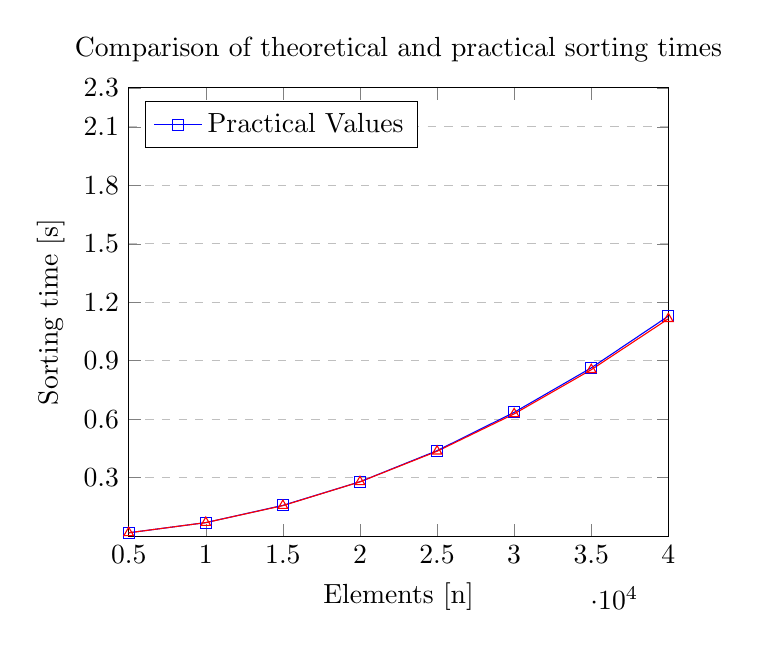
\begin{tikzpicture}
\begin{axis}[
    title={Comparison of theoretical and practical sorting times},
    xlabel={Elements [n]},
    ylabel={Sorting time [s]},
    xmin=5000, xmax=40000,
    ymin=0, ymax=2.3,
    xtick={0,5000,10000,15000,20000,25000,30000,35000,40000},
    ytick={0.3,0.6,0.9,1.2,1.5,1.8,2.1,2.3},
    legend pos=north west,
    ymajorgrids=true,
    yminorgrids=true,
    grid style=dashed,
]

\addplot[
    color=blue,
    mark=square,
    ]
    coordinates {
    (5000,0.017429)(10000,0.0697857)(15000,0.158103)(20000,0.279351)(25000,0.438815)(30000,0.635349)(35000,0.863602)(40000,1.12893)
   
    };
    \legend{Practical Values}

\addplot[
    color=red,
    mark=triangle,
    ]
    coordinates {
    (5000,0.017429)(10000,0.069716)(15000,0.156861)(20000,0.278864)(25000,0.435725)(30000,0.627444)(35000,0.854021)(40000,1.115456)
    };
  
\end{axis}
\end{tikzpicture}
\end{center}

\subsubsection{QuickSort}
\begin{center}
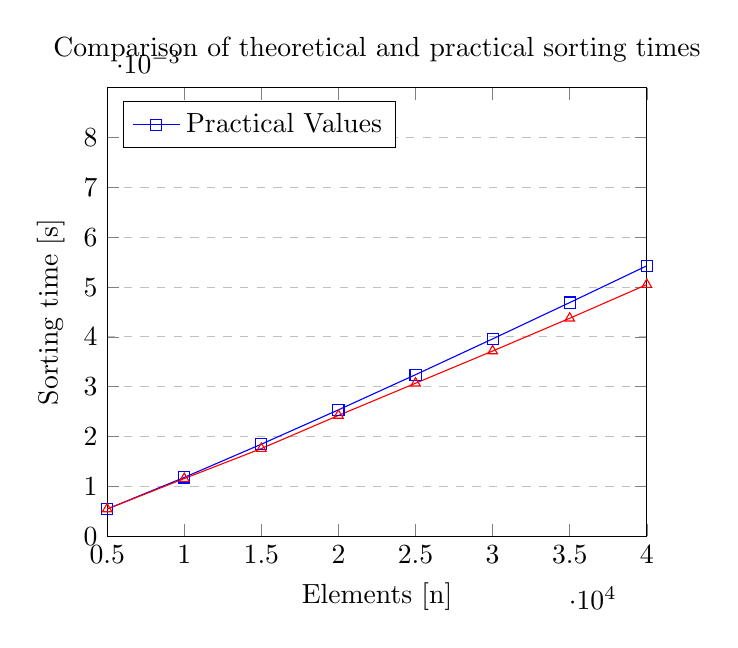
\begin{tikzpicture}
\begin{axis}[
    title={Comparison of theoretical and practical sorting times},
    xlabel={Elements [n]},
    ylabel={Sorting time [s]},
    xmin=5000, xmax=40000,
    ymin=0, ymax=0.009,
    xtick={0,5000,10000,15000,20000,25000,30000,35000,40000},
    ytick={0,0.001,0.002,0.003,0.004,0.005,0.006,0.007,0.008},
    legend pos=north west,
    ymajorgrids=true,
    yminorgrids=true,
    grid style=dashed,
]

\addplot[
    color=blue,
    mark=square,
    ]
    coordinates {
    (5000,0.000545385)(10000,0.0011795391676292309)(15000,0.001847198702868842)(20000,0.0025366166705169235)(25000,0.003242214060695192)(30000,0.003960704908625377)(35000,0.004689917958848073)(40000,0.00542831001155077)
   
    };
    \legend{Practical Values}

\addplot[
    color=red,
    mark=triangle,
    ]
    coordinates {
    (5000,0.000545385)(10000,0.00115669)(15000,0.00175919)(20000,0.0024239)(25000,0.00307048)(30000,0.00371731)(35000,0.00437498)(40000,0.00505177)
    
    };
  
\end{axis}
\end{tikzpicture}
\end{center}

\begin{center}
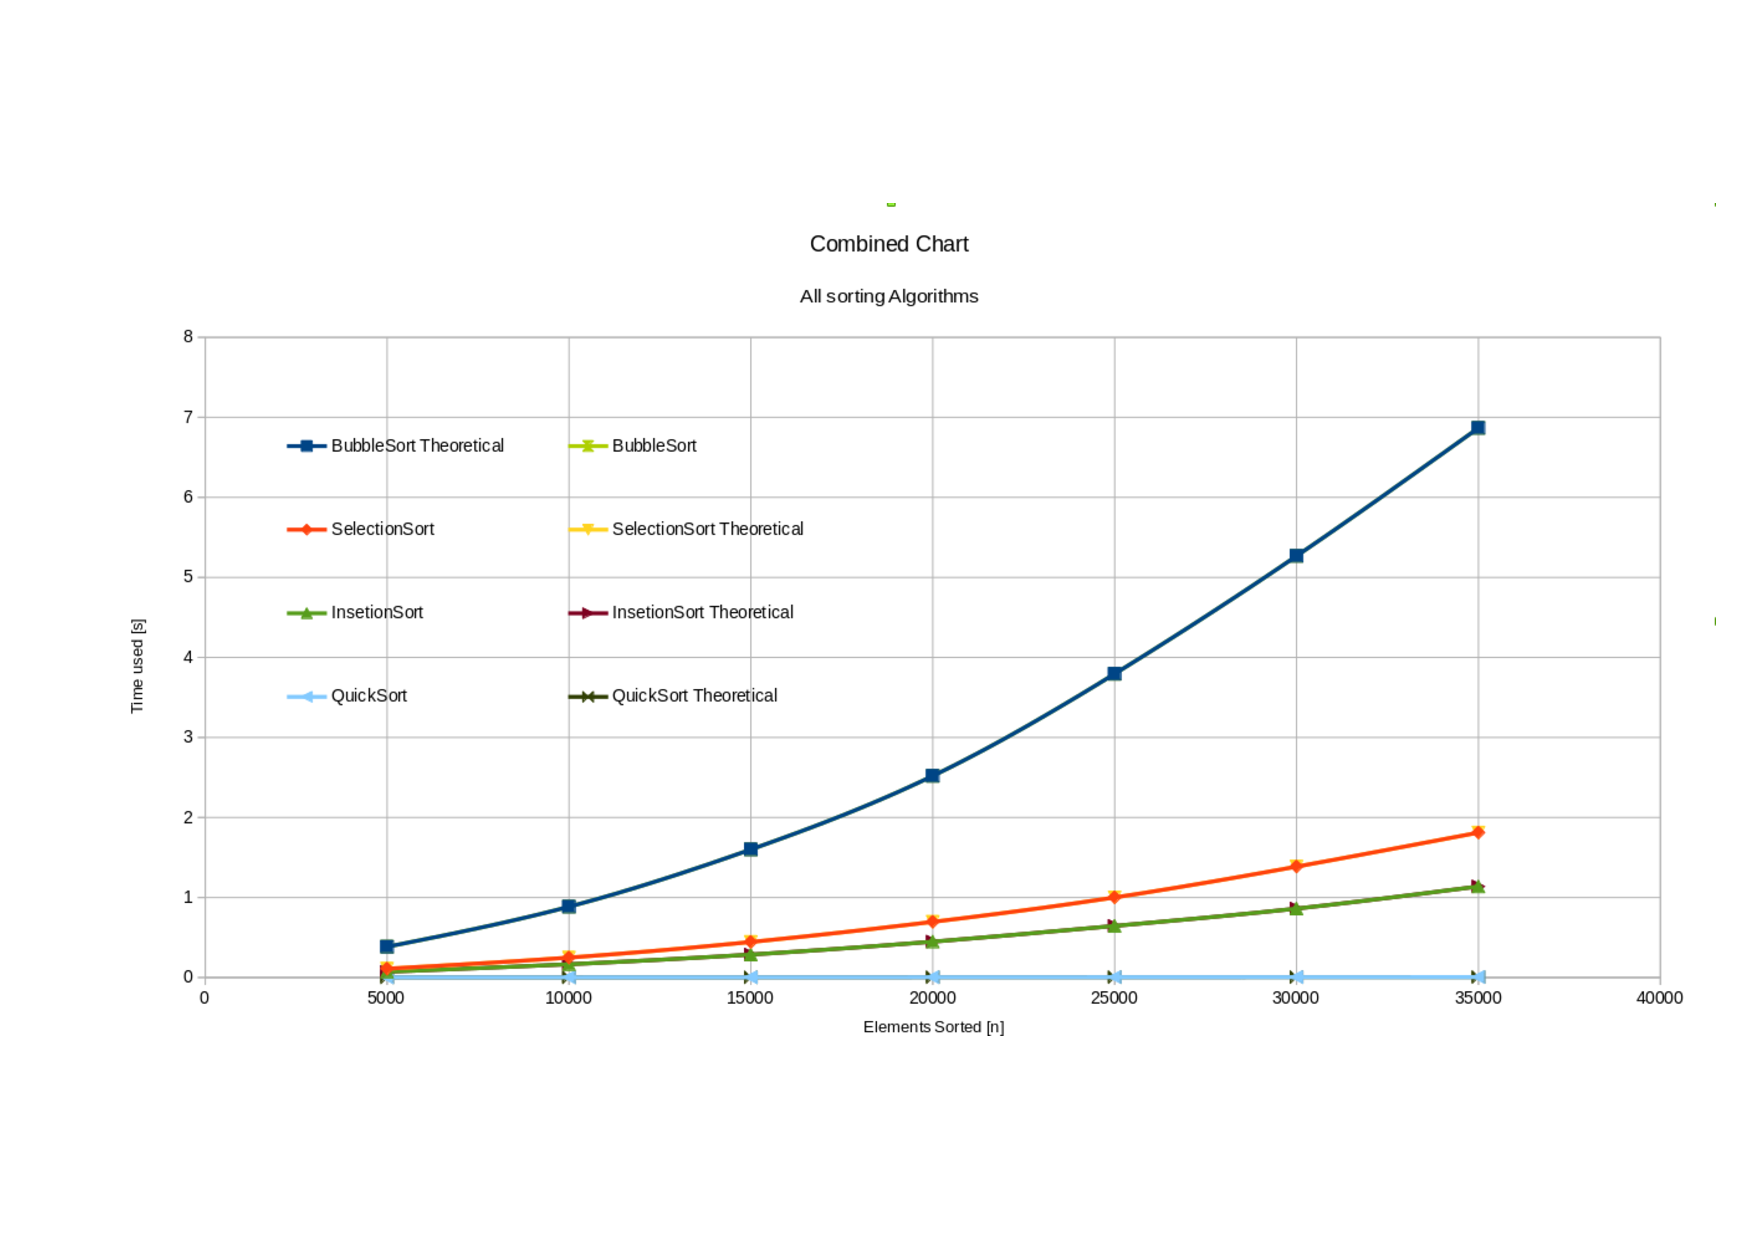
\includegraphics[scale=0.5]{Image}
\end{center}




Here we see that in everyway imagenable. That amongst the sorting algorithms we tested, Quicksort rules them all.

\section{Enviroment}
I'm programming on an Arch Linux 64-bit system. I've got the c++ compiler installed and compile using it's g++ alias which links necessary libraries automatically. To compile i use the recommended flags: "-std=c++11 -Wall -pedantic". The flags let me choose to use c++11 standard and give me useful compiling warnings and errors. 
\flushright{\today}
\end{document}
